\providecommand{\main}{../../..}
\documentclass[\main/main.tex]{subfiles}
\begin{document}

\subsection{Esercizio 3}
Dato il problema di programmazione a due obbiettivi:

\begin{align*}
  \max f_1(x)          & = x_1 - 2x_2                                          \\
  \max f_2 (x)         & = x_2                                                 \\
  \text {con } x \in X & = \{x:2x_1+x_2\leq 5; 0 \leq x_1 \leq 2; x_2 \geq 0\}
\end{align*}

\begin{enumerate}[a)]
  \item Si ricavi la regione paretiana con il metodo dei vincoli (sostituendo la seconda funzione obiettivo con un vincolo) e la si disegni nello spazio delle variabili $x_1 - x_2$ e in quello degli obiettivi $f_1 - f_2$.
  \item Si determini graficamente la soluzione ottima con il metodo dei pesi, ponendo i pesi dei due obiettivi pari rispettivamente ad $\alpha_1 = \alpha_2 = \frac{1}{2}$.
\end{enumerate}

\subsection{Soluzione esercizio 3}
\subsubsection*{Riscrivo il problema}
La funzione obbiettivo $f_2$ è da massimizzare, per cui il vincolo che costruisco è $f_2 \geq \epsilon_2$.

\begin{align*}
  \max f_1(x)          = x_1 - 2x_2 \\
  x_2        & \geq \epsilon_2      \\
  2x_1+x_2   & \leq 5               \\
  0 \leq x_1 & \leq 2               \\
  x_2        & \geq 0
\end{align*}

\subsubsection*{Dominio del problema}

\begin{figure}
  \begin{subfigure}{0.45\textwidth}
    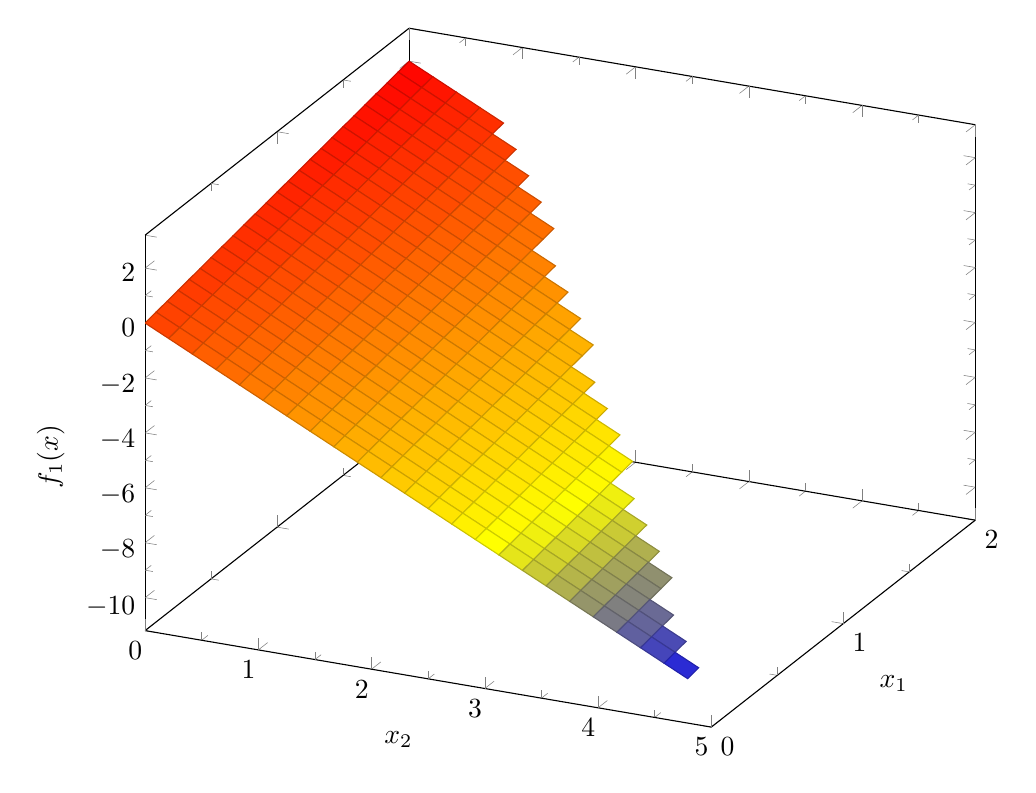
\begin{tikzpicture}
      \begin{axis}[
          width= \textwidth,
          xlabel=$x_2$,
          ylabel=$x_1$,
          zlabel=$f_1(x)$,
          y domain=0:2,
          domain=0:5,
          ztick = {-10,-8,...,2},
          xtick = {0,...,5},
          ytick = {0,1,2},
          ymin=0,
          xmin=0,
          ymax=2,
          xmax=5,
          minor tick num=1
        ]
        \addplot3[surf, unbounded coords=jump]{2*y+x<=5 && x >= 0 && y <= 2 && y >= 0? y-2*x : NaN};
      \end{axis}
    \end{tikzpicture}
    \caption{La funzione $f(x)$}
    \label{func_1}
  \end{subfigure}
  ~
  \begin{subfigure}{0.45\textwidth}
    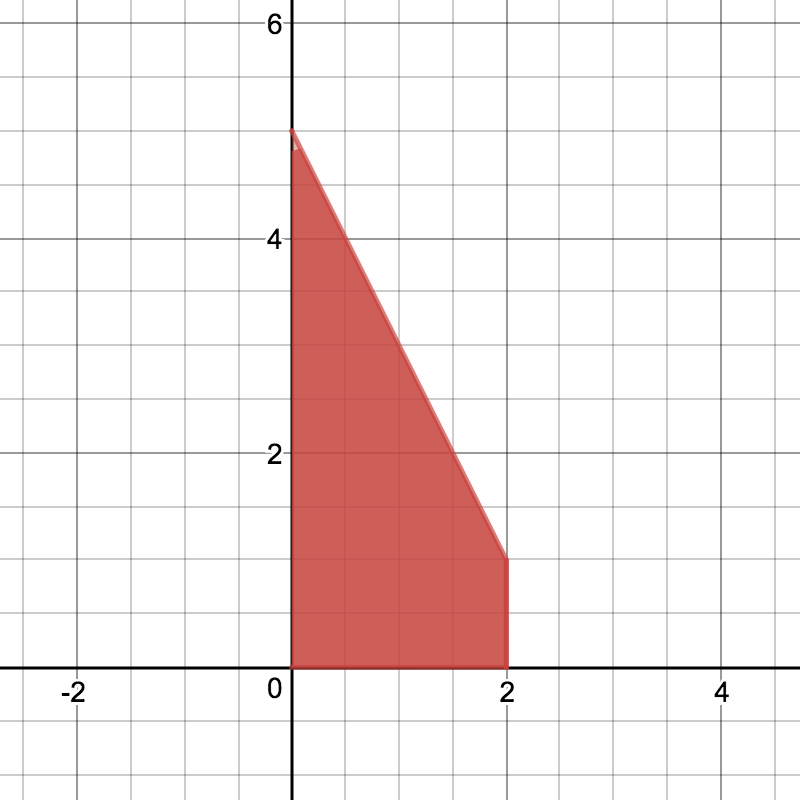
\includegraphics[width=0.8\textwidth]{11042017-1}
    \caption{Dominio della funzione $f_1(x)$}
  \end{subfigure}
\end{figure}

\subsubsection*{Identifico lo standard $\epsilon_2$}
Al variare del parametro $\epsilon_2$ nel dominio di interesse $[0,5]$ la funzione obbiettivo $f_1$ assume il massimo inizialmente in $(0,5)$, quindi si sposta sul segmento di destra sino al punto $(1,2)$ ed infine si sposta gradualmente sino a $(0,2)$.

\begin{figure}
  \begin{subfigure}{0.45\textwidth}
    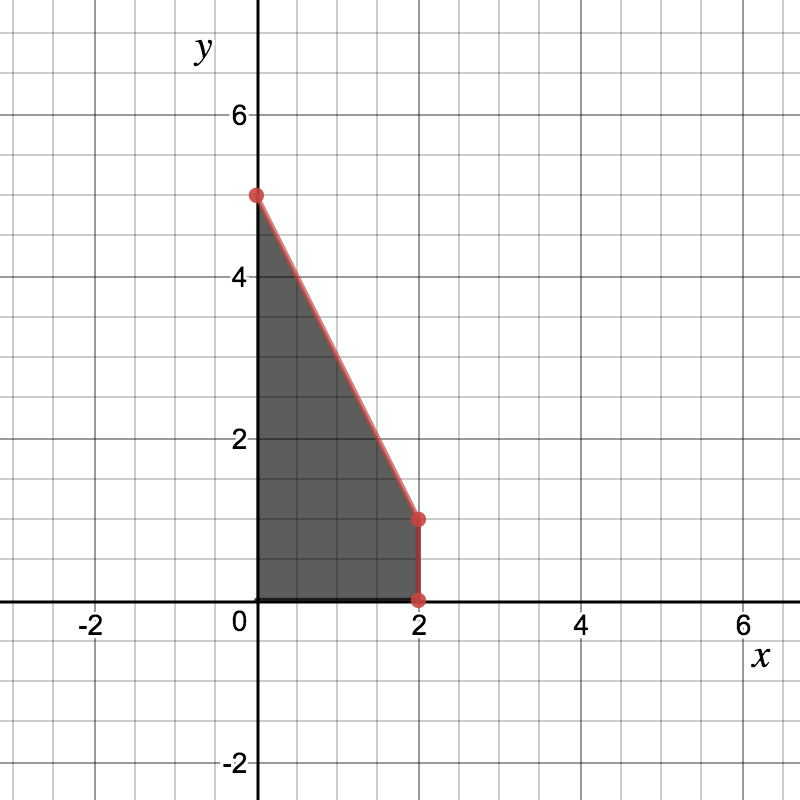
\includegraphics[width=0.8\textwidth]{11042017-2}
    \caption{Regione paretiana nello spazio $x_1, x_2$}
  \end{subfigure}
  \begin{subfigure}{0.45\textwidth}
    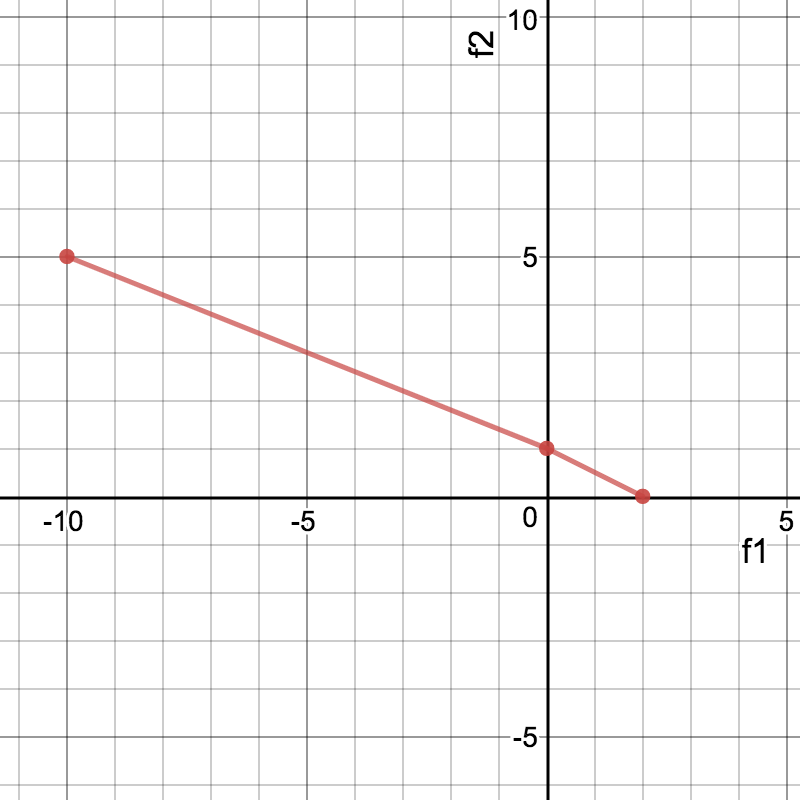
\includegraphics[width=0.8\textwidth]{11042017-3}
    \caption{Regione paretiana nello spazio $f_1, f_2$}
  \end{subfigure}
\end{figure}

\subsubsection*{Risoluzione con metodo dei pesi}
\[
  \frac{1}{2}(x_1 - 2x_2) + \frac{1}{2}(x_2) = \frac{1}{2}(x_1 - 2x_2 + x_2) = \frac{1}{2}(x_1 - x_2)
\]

Il punto di massimo assunto dalla funzione del dominio di definizione è pari a $(\max(x_1), \min(x_2))$, cioè $(2,0)$ che fa parte della regione paretiana identificata al punto precedente.
\end{document}